\documentclass[11pt]{beamer}
\usepackage[utf8]{inputenc}
\usepackage[T1]{fontenc}
\usepackage{lmodern}
\usetheme{Berlin}
\begin{document}
\author[{Team No-1086}]{
\\ \textbf{Team members:
	Catherine Monisha E.}\vspace{8pt}\\ \textbf{Nirmala R.}\vspace{8pt}
\\ \textbf{Veni Gayathri S.}\vspace{8pt}
\\ \textbf{Atchaya A.}\vspace{8pt}\\ \textbf{Guided By: Mr.Rajkumar K.}}
\title{eYIC Project Proposal 2019-2020}
\subtitle{BACK TO NATURE}
%\logo{}
\institute{SRI SAI RAM ENGINEERING COLLEGE}
\date{\today}
\setbeamercovered{transparent}
\setbeamertemplate{navigation symbols}{}
\frame{\titlepage}
\begin{frame}
\frametitle{Introduction}
\textbf{Problem Domain: Responsible Consumption and Production}
\\ \textparagraph
Food waste or food loss is food that is wasted, lost or uneaten. 
 The causes of food waste or loss are numerous and occur at the stages of producing, processing, retailing and consuming.
\\ \textparagraph
Effects of food waste are:
Wastage of fertile land,freshwater,Biodiversity loss
,Increased carbon footprint
\\ \textparagraph
	 Besides the effort required to collect and dispose of it, food waste contaminates the environment,causes odour nuisance and compromises recycling efforts.
\\ \textparagraph
	Food producers can solve their food waste problems by simply organizing an effective composting strategy. 
\end{frame}
\begin{frame}
	\frametitle{Description}
\\ \textparagraph
'Back To Nature' is a revolutionary device that turns food scraps into fertilizer.
Designed to fit seamlessly into our kitchen, the elegant household compost machine easily converts food waste into ready-to-use, homemade fertilizer.
It collects food scraps throughout the week, and then uses a combination of heat, moisture and mechanical agitation to turn the waste into compost, all in an impressive 24 hours. 
\\ \textbf{FEASIBILITY:}
 \textparagraph 
Being a compact,user friendly device with elegent design,this food recycler will find its place in every kitchen instantly.It also comes at an affordable price and provides return on investment.
\end{frame}	
\begin{frame}
\frametitle{Market Research}
\begin{itemize}
	\item Weddings, canteens, hotels, social and family functions, households spew out so much food. According to the United Nations Development Programme, up to 40\% of the food produced in India is wasted. 
	India wastes Rs 244 crore worth of food a day.
	\item The civic body, quoting the Solid Waste Management rules, 2016, instructed all restaurant owners to dispose their waste- by setting up composting sites on their premises. On the other hand, hotel association members are quoting the Food safety and standards Act, according to which they can’t compost on their premises.
\end{itemize}	
\end{frame}
\begin{frame}
	\begin{itemize}
	\item The group of restaurateurs opined that the solution to Mumbai’s restaurants waste management lies in micro management rather than large scale plans. 75\% of the restaurants have 10\%-20\% extra preparation.
	\item It’s time for action — and in particular viable actions on SDG12 and the target of reducing food loss and halving food waste by 2030.
\end{itemize}
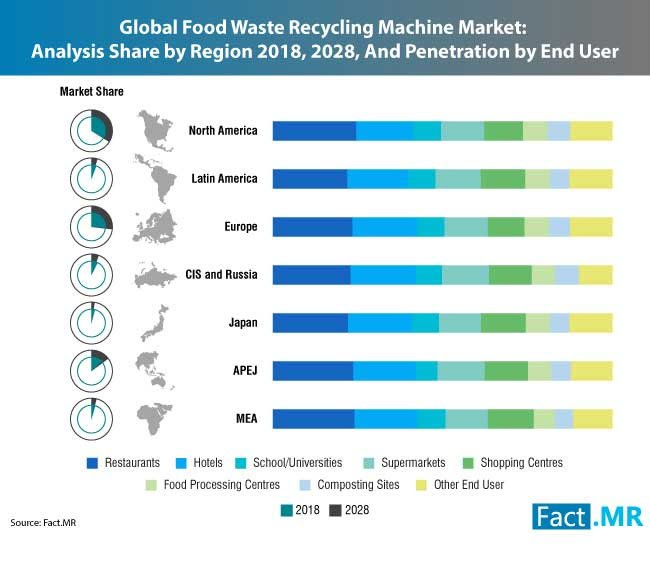
\includegraphics[height=0.45\textheight]{market.jpeg}
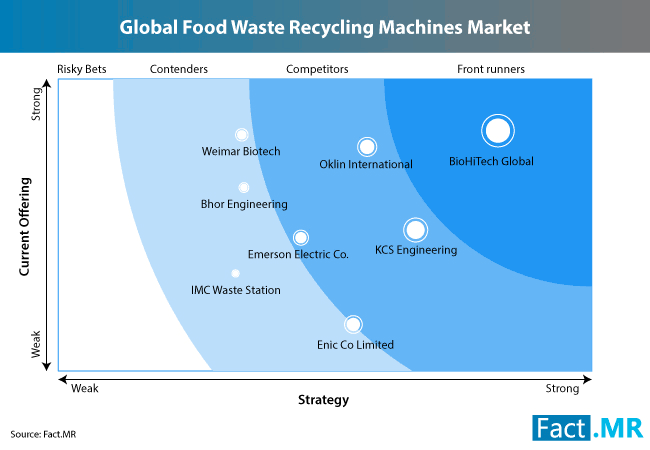
\includegraphics[width=0.65\textheight]{market1.jpeg}
	\end{frame}
\begin{frame}
\frametitle{Implementation}
\begin{itemize}
\item Open the lid to push the food waste, which could be anything from peels to leftover meat, and shut the lid.\item When the bin reaches full capacity, press the start button.\item When the moisture in the wet waste is sensed by the humidity sensor, the blades starts mixing and rotate at the speed of 2 RPM.\item Heater turns ON and composting tank becomes hot.Water content in the wet waste is evaporated and it goes out to the atmosphere as water vapour through exhaust system.(70-75\% volume reduction of waste)
\end{itemize}
\end{frame}
\begin{frame}
	\frametitle{Working}
	\begin{itemize}	
	\item At the same time micro organisms decompose organic waste into compost in 24 hours.(80-95\% volume reduction) \item After removing  the compost , preserve it for certain days.Now, we have obtained usable fertilizer within 24 hrs which can be used for farming or home garden.  
	\end{itemize}
 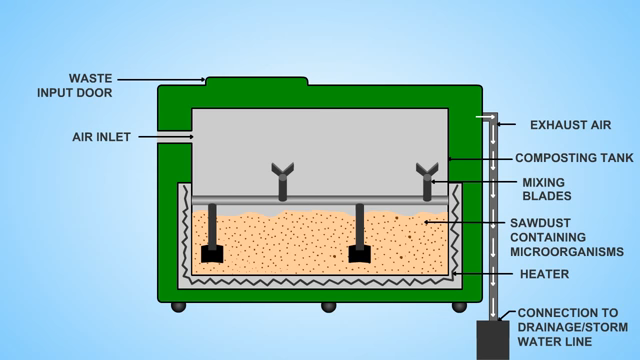
\includegraphics[height=0.35\textheight]{img.png}
 \hfill
 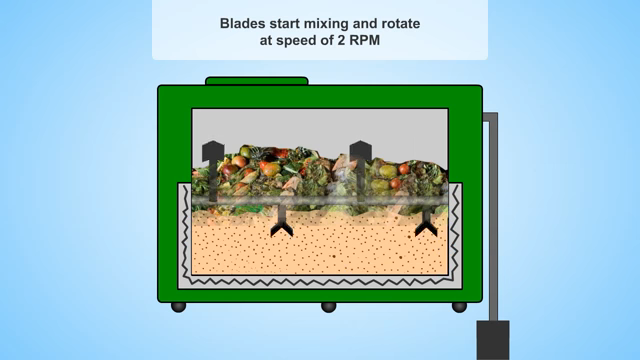
\includegraphics[height=0.35\textheight]{img1.png}
\end{frame}
\begin{frame}
	\frametitle{Components}
	\\ \textbf{HARDWARE REQUIREMENTS:}
	\\ \textbf{COST ANALYSIS:}
\end{frame}

\end{document}	
